\documentclass[12pt]{article}
\usepackage[polish]{babel}
\usepackage[utf8]{inputenc}
\usepackage{array}
\usepackage{float}
\usepackage{graphicx} % Add this line to include graphics
\graphicspath{ {./assets/} }

\title{SPD Lab 1 Głośność}
\author{Krzysztof Rudnicki, 307585}
\date{\today}

\begin{document}

\maketitle


\section{Krzywe poziomu głośności}
\begin{center}
    \begin{tabular}{ | >{\arraybackslash}m{3cm} | l | l | l | l | l | l | l | l | } 
      \hline
      & \multicolumn{8}{c|}{Częstotliwość f tonu regulowanego (Hz)} \\ \hline
      Poziom tonu odniesienia 1000 Hz (dB) & 125 & 250 & 500 & 1000 & 1500 & 2000 & 3000 & 4000 \\ 
      \hline
      40 & 62 & 52 & 46 & 40 & 32 & 34 & 26 & 40 \\ 
      \hline
      60 & 62 & 56 & 58 & 60 & 50 & 46 & 38 & 52 \\ 
      \hline
      80 & 78 & 70 & 78 & 80 & 74 & 70 & 58 & 68 \\ 
      \hline
    \end{tabular}
    \end{center}
    \begin{figure}[H]
        \centering
        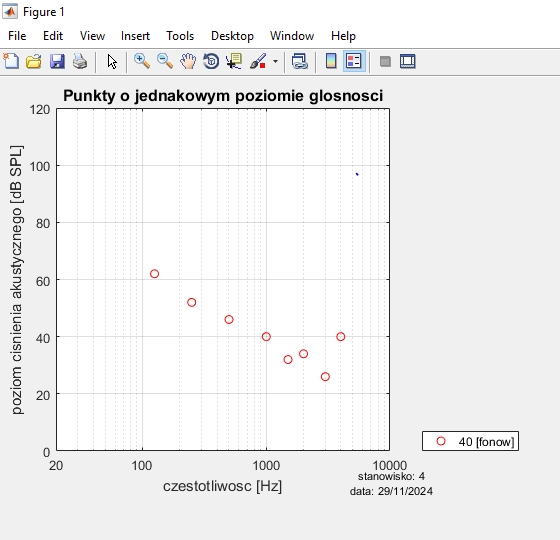
\includegraphics[width=\textwidth]{glosnosc_40.png}
        \caption{Krzywa poziomu głośności dla 40 dB}
    \end{figure}
    \begin{figure}[H]
        \centering
        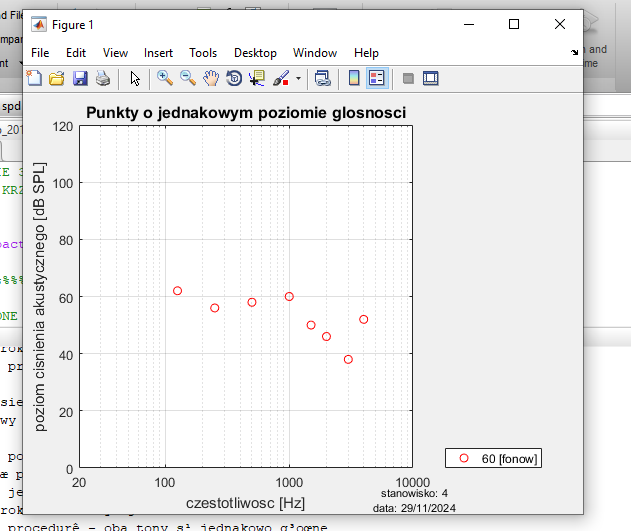
\includegraphics[width=\textwidth]{glosnosc_60.png}
        \caption{Krzywa poziomu głośności dla 60 dB}
    \end{figure}
    \begin{figure}[H]
        \centering
        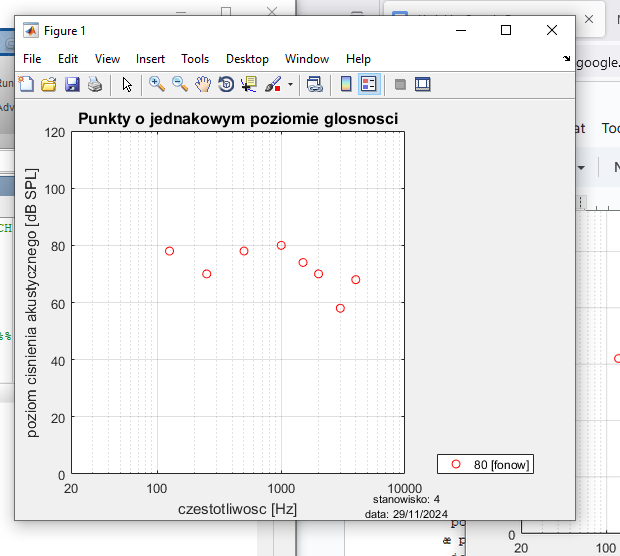
\includegraphics[width=\textwidth]{glosnosc_80.png}
        \caption{Krzywa poziomu głośności dla 80 dB}
    \end{figure}

\newpage
\section{Sony}
Poziomy [fony] Poziomy [dB] i macierz ocen:
\begin{verbatim}
ans =
  Columns 1 through 11
   30.0000   30.0083   30.0000   30.0000   30.0000   
   30.0000   30.0000   30.0000   30.0000   33.0000   
   30.0000   40.0000   40.0100   35.0000   30.0000   
   35.0000   30.0000   35.0000   30.0000   30.0000   
   30.0000   35.0000   50.0000   50.0110   50.0000   
   30.0000   40.0000   35.0000   35.0000   40.0000   
   40.0000   35.0000   40.0000   60.0000   60.0116   
   0.0000    35.0000   41.0000   46.0000   40.0000   
   50.0000   49.0000   40.0000   40.0000   70.0000   
   70.0119   40.0000   40.0000   45.0000   45.0000   
   50.0000   70.0000   45.0000   50.0000   60.0000
   80.0000   80.0121   80.0000   65.0000   75.0000   
   75.0000   56.0000   50.0000   50.0000   55.0000   
   55.0000

  Columns 12 through 22
   30.0000   30.0000   28.0000   30.0000   32.0000   
   30.0000   25.0000   30.0000   30.0000   30.0000   
   29.0000   39.0000   30.0000   40.0000   30.0000   
   35.0000   30.0000   30.0000   35.0000   30.0000   
   35.0000   33.0000   30.0000   39.0000   38.0000   
   30.0000   35.0000   35.0000   30.0000   45.0000   
   40.0000   39.0000   30.0000   33.0000   35.0000   
   40.0000   35.0000   35.0000   40.0000   40.0000   
   35.0000   38.0000   55.0000   30.0000   40.0000   
   55.0000   45.0000   45.0000   40.0000   40.0000   
   60.0000   40.0000   45.0000   48.0000   65.0000
   50.0000   60.0000   78.0000   78.0000   45.0000   
   45.0000   80.0000   70.0000   55.0000   75.0000   
   60.0000

  Columns 23 through 32
   30.0000   29.0000   28.0000   30.0000   29.0000   
   29.0000   30.0000   30.0000   30.0000   30.0000
   30.0000   30.0000   40.0000   38.0000   30.0000   
   30.0000   35.0000   29.0000   30.0000   40.0000
   40.0000   40.0000   37.0000   30.0000   30.0000   
   35.0000   36.0000   35.0000   30.0000   40.0000
   40.0000   40.0000   45.0000   39.0000   45.0000   
   60.0000   40.0000   50.0000   36.0000   35.0000
   40.0000   45.0000   55.0000   40.0000   42.0000   
   45.0000   50.0000   60.0000   45.0000   5.0000
   65.0000   75.0000   50.0000   45.0000   70.0000   
   65.0000   55.0000   70.0000   70.0000   60.0000
\end{verbatim}
\begin{figure}[H]
    \centering
    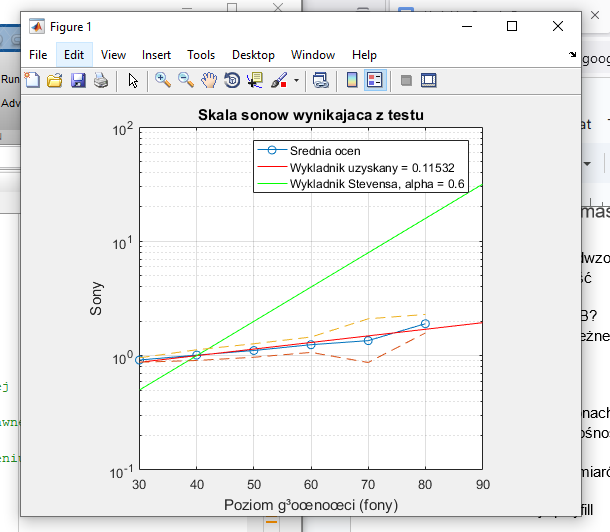
\includegraphics[width=\textwidth]{sony.png}
    \caption{Macierz ocen Sony}
\end{figure}
\begin{table}[H]
\centering
\begin{tabular}{|c|c|c|c|c|}
\hline
Poziomy [fony] & Poziomy [dB] & Oceny średnie & Zakres minus & Zakres plus \\ \hline
30.0000 & 30.0083 & 29.7054 & 28.4096 & 31.0602 \\ \hline
40.0000 & 40.0100 & 32.7776 & 29.4227 & 36.5149 \\ \hline
50.0000 & 50.0110 & 35.9764 & 31.4093 & 41.2075 \\ \hline
60.0000 & 60.0116 & 40.4154 & 34.6291 & 47.1686 \\ \hline
70.0000 & 70.0119 & 43.8832 & 28.2547 & 68.1563 \\ \hline
80.0000 & 80.0121 & 61.7038 & 51.2020 & 74.3595 \\ \hline
\end{tabular}
\end{table}

\begin{table}[H]
\centering
\begin{tabular}{|c|c|c|c|c|}
\hline
Poziomy [fony] & Poziomy [dB] & Wartości w sonach & Zakres minus & Zakres plus \\ \hline
30.0000 & 30.0083 & 0.9163 & 0.8764 & 0.9581 \\ \hline
40.0000 & 40.0100 & 1.0111 & 0.9076 & 1.1264 \\ \hline
50.0000 & 50.0110 & 1.1098 & 0.9689 & 1.2712 \\ \hline
60.0000 & 60.0116 & 1.2467 & 1.0682 & 1.4550 \\ \hline
70.0000 & 70.0119 & 1.3537 & 0.8716 & 2.1025 \\ \hline
80.0000 & 80.0121 & 1.9034 & 1.5795 & 2.2938 \\ \hline
\end{tabular}
\end{table}

\section{$\Delta L$}
\subsection{$\Delta L$ szum}
\begin{figure}[H]
    \centering
    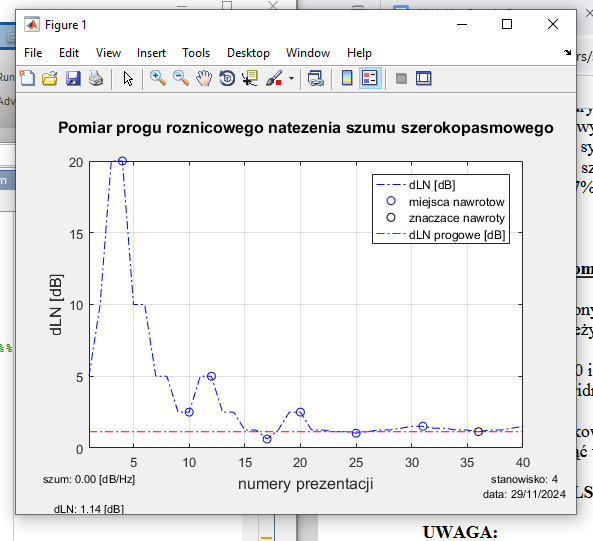
\includegraphics[width=\textwidth]{szum_0.png}
    \caption{$\Delta L$ szum 0 dB}
\end{figure}
\begin{figure}[H]
    \centering
    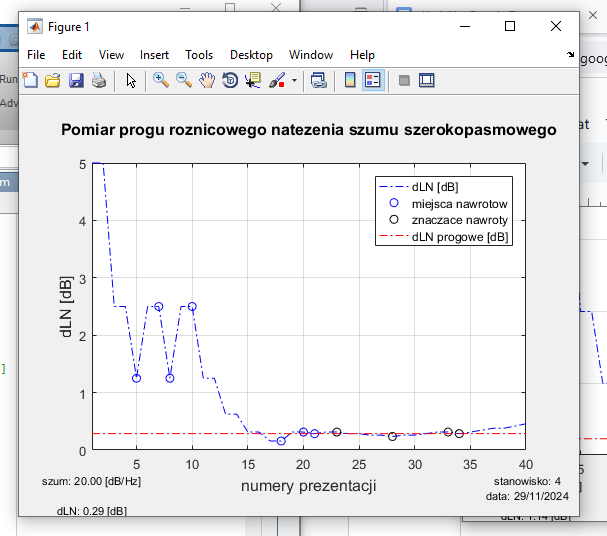
\includegraphics[width=\textwidth]{szum_20.png}
    \caption{$\Delta L$ szum 20 dB}
\end{figure}
\begin{figure}[H]
    \centering
    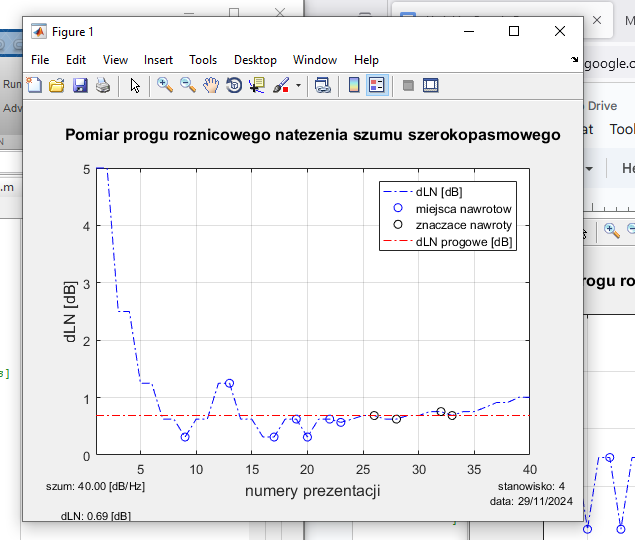
\includegraphics[width=\textwidth]{szum_40.png}
    \caption{$\Delta L$ szum 40 dB}
\end{figure}

\subsection{$\Delta L$ ton}
\begin{figure}[H]
    \centering
    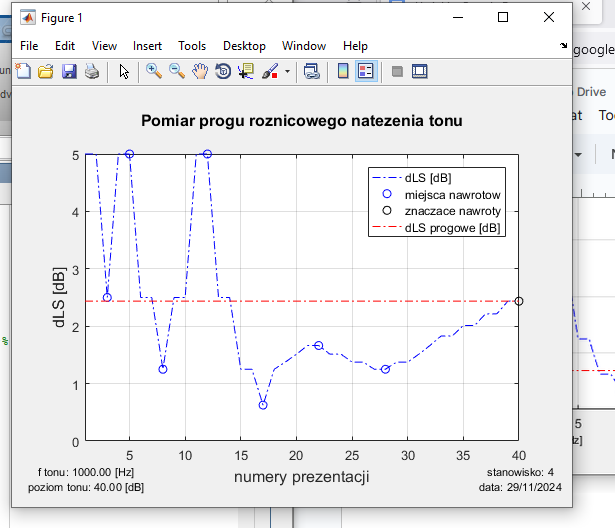
\includegraphics[width=\textwidth]{ton_40.png}
    \caption{$\Delta L$ ton 40 dB}
\end{figure}
\begin{figure}[H]
    \centering
    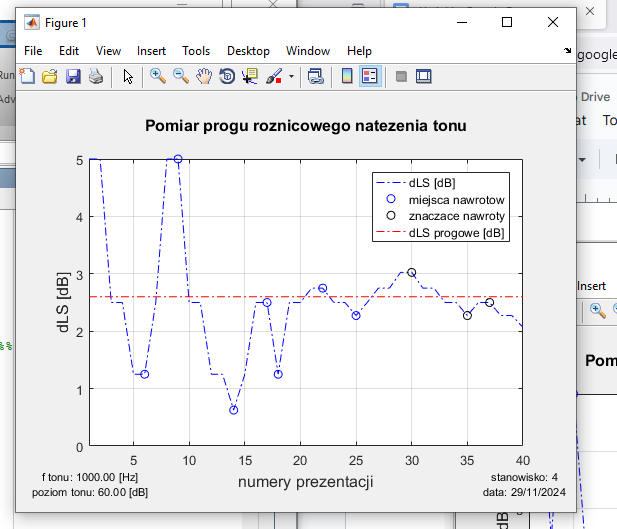
\includegraphics[width=\textwidth]{ton_60.png}
    \caption{$\Delta L$ ton 60 dB}
\end{figure}
\begin{figure}[H]
    \centering
    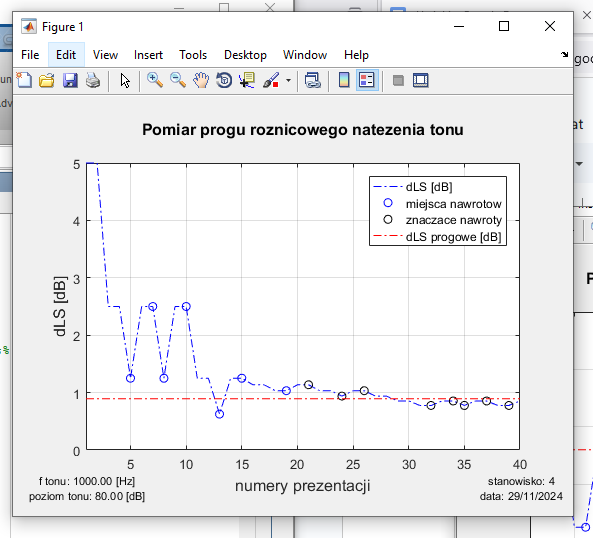
\includegraphics[width=\textwidth]{ton_80.png}
    \caption{$\Delta L$ ton 80 dB}
\end{figure}

\end{document}